\documentclass[11pt]{article}

\usepackage[utf8]{inputenc}
\usepackage[T1]{fontenc}
\usepackage{lmodern}
\usepackage[margin=1in]{geometry}
\usepackage{amsmath,amssymb}
\usepackage{booktabs}
\usepackage{tabularx}
\usepackage{array}
\usepackage{enumitem}
\usepackage{fvextra}
\usepackage{newunicodechar}
\usepackage{tikz}
\usetikzlibrary{arrows.meta,positioning,fit,backgrounds}
\usepackage[numbers,sort&compress]{natbib}
\usepackage[hidelinks]{hyperref}

\newunicodechar{≠}{\ensuremath{\neq}}
\newunicodechar{∧}{\ensuremath{\wedge}}
\newunicodechar{→}{\ensuremath{\to}}
\newunicodechar{∀}{\ensuremath{\forall}}

\newcommand{\code}[1]{\texttt{#1}}
\newcommand{\lean}[1]{\texttt{#1}}

\title{CogLean: Compositional Proof of Cognitive Predictions}
\author{Jeff Shrager}
\date{Draft for circulation, October 2026}

\begin{document}
\sloppy
\maketitle

\begin{abstract}
Cognitive science has many computational theories, but little cumulative theoretical knowledge. Theories are implemented as separate programs, so combining two of them usually means writing a third, and what a theory predicts is usually established by running it. We describe CogLean, a library of cognitive theory in the Lean proof assistant, organized on the model of Mathlib, the community library of formalized mathematics. CogLean is not a new theory of cognition. Its shared library, CogLib, holds representations, mechanisms, theory-neutral statements of phenomena, and theorems about them. Existing theories are expressed as choices of those mechanisms, and their consequences are proved, not simulated.

The central demonstration composes two independently formalized theories: EPAM's discrimination-net recognition (Feigenbaum and Simon) and the distributions-of-associations model of strategy choice (Siegler and Shrager). They are joined with a problem solver in the GPS and repair-theory tradition to produce a model of three-digit addition. Every component, and every theorem about it, was established before the composition. The composed model computes all of its answers; no route is given the correct sum. Its predictions are proved by reusing those theorems. One is the \emph{confident error}: a problem confused with a familiar one gets the familiar problem's answer, wrongly, with no more use of the backup procedure than the familiar problem itself. Neither theory makes this prediction alone. Others say that improving the fallback solver cannot reduce such errors, and that a confused problem has two sources of error with different signatures. Replacing EPAM's memory with ACT-R's declarative memory, and changing nothing else, changes these predictions, and laws of memory that one memory has and the other lacks explain why.

We separate results that hold for every setting of the mechanisms from results that need stated conditions, and both from exact values at illustrative settings. We also report what an independent, blind simulation found that the proofs did not: hypotheses that learned networks never reach, and an unstated assumption on which a predicted learning sequence depends.
\end{abstract}

\section{Introduction}

Cognitive science has accumulated many computational theories of memory, learning, problem solving and skill. It has accumulated much less theory that can be \emph{reused}. A theory of memory developed for verbal learning usually has to be reimplemented before it can take part in a model of arithmetic. When two theories are combined, the result is a new program, whose behavior must be explored afresh by simulation. Newell's complaint that the field asks nature twenty questions without assembling the answers \citep{newell1973}, and his call for unified theories \citep{newell1990}, are about this problem. So, more recently, are arguments that computational modeling forces theories to be made explicit \citep{guest2021} and that psychology needs explanatory theories, not only tests \citep{vanrooij2021}.

Mathematics faced a version of the same problem and has made progress on it. Mathlib \citep{mathlib2020}, the community library of formalized mathematics for the Lean proof assistant \citep{demoura2021}, does not propose new mathematics. It provides one shared formal environment, in which definitions are made once, every result is machine-checked, and later work builds on earlier results by citing them. A theorem about groups, once proved, is available to everyone who uses groups.

This paper asks whether the same organization can work for cognitive theory:

\begin{quote}
\emph{If independently developed cognitive theories are represented in a common formal library, can we derive scientifically meaningful consequences from their composition, consequences that would otherwise require building and investigating a new integrated model from scratch?}
\end{quote}

We describe CogLean \citep{coglean}, an initial library built to test this, and give a concrete, checked answer in one case. The case is three-digit addition, composed from EPAM's discrimination nets \citep{feigenbaum1959,feigenbaum1962}, Siegler and Shrager's distributions-of-associations (DOA) model of strategy choice \citep{siegler1984}, and a problem solver in the tradition of GPS and repair theory \citep{newell1972,brown1980}. Arithmetic is the demonstration, not the objective. We are not proposing a new theory of children's arithmetic. Multi-digit addition is a familiar task, complex enough to need several mechanisms, and two of the needed theories already exist.

The argument is organized around three capabilities, in increasing order of importance.
\begin{enumerate}
  \item \textbf{Formalization.} Existing theories are stated as definitions, postulates and theorems. Each theorem's assumptions are explicit.
  \item \textbf{Composition.} Formalized mechanisms are reused in new contexts, and so are the \emph{theorems} about them. A library of reusable cognitive algorithms would be useful software. A library of reusable \emph{results} is a contribution to theory.
  \item \textbf{Discovery.} Composition establishes consequences that the original theories' authors did not state. Formalization also exposes unstated assumptions, results that depend on parameters, results that hold for whole classes of models, and conditions under which theories diverge.
\end{enumerate}

A caution belongs at the start. Lean checks that each conclusion follows from its premises. It does not check that the premises describe people, nor that a valid derivation is an explanation. Section~\ref{sec:status} takes this up directly, and we distinguish throughout what holds generally, what holds under stated conditions, and what was computed at illustrative settings.

\section{CogLean}
\label{sec:coglean}

\subsection{Organization}

CogLean has four layers (Figure~\ref{fig:arch}).
\begin{itemize}
  \item \textbf{Lean}, the formal language and proof checker. CogLean uses only Lean's core, not Mathlib, and every probability is an exact rational number.
  \item \textbf{CogLib}, the general library. It holds:
  \begin{itemize}
    \item representations: feature codes, finite probability distributions, semantic networks;
    \item memory structures: discrimination nets, an ACT-R-style activation memory;
    \item processes: discrimination learning, sampled retrieval with a confidence criterion, ``recognize, then retrieve, else back up'', and a decision cycle with impasses and repairs;
    \item an interface any memory can implement (a \emph{retriever}: study an item, retrieve a distribution over stored items);
    \item theory-neutral statements of phenomena and laws, such as the serial-position effect, or the law that retrieval of a studied item is certain.
  \end{itemize}
  CogLib imports no theory.
  \item \textbf{Theories}, each a package that states its postulates as choices of CogLib constructs, cited to their sources, and proves its phenomena.
  \item \textbf{Applications}, models of particular tasks assembled from theories and library mechanisms, with the task's own knowledge.
\end{itemize}

\begin{figure}[t]
\centering
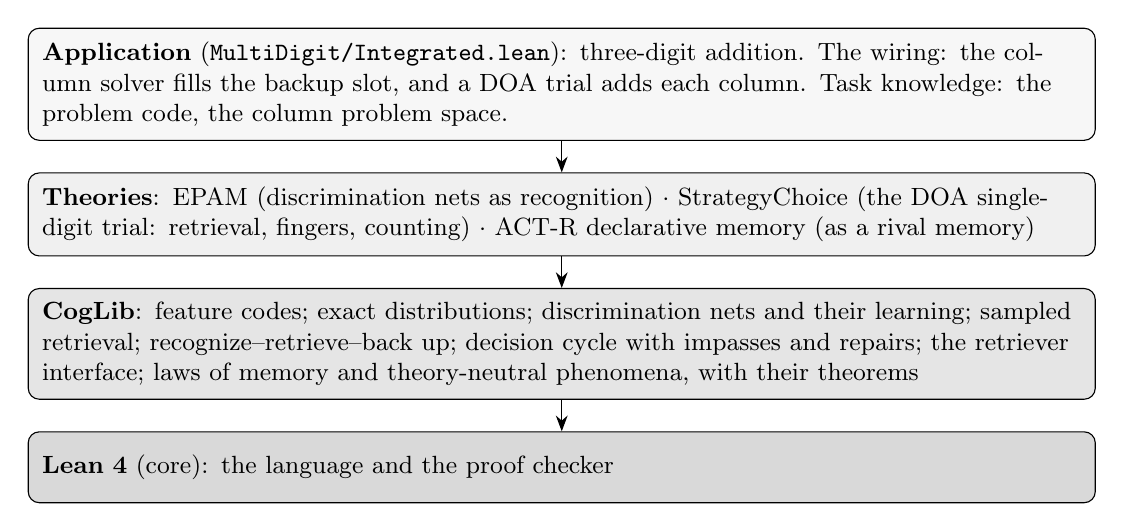
\begin{tikzpicture}[font=\small,
  layer/.style={draw, rounded corners, minimum height=9mm, text width=13.2cm, align=left, inner sep=5pt},
  arr/.style={-{Stealth[length=2mm]}}]
  \node[layer, fill=black!3] (app) {\textbf{Application} (\code{MultiDigit/Integrated.lean}): three-digit addition. The wiring: the column solver fills the backup slot, and a DOA trial adds each column. Task knowledge: the problem code, the column problem space.};
  \node[layer, fill=black!6, below=4mm of app] (th) {\textbf{Theories}: EPAM (discrimination nets as recognition) $\cdot$ StrategyChoice (the DOA single-digit trial: retrieval, fingers, counting) $\cdot$ ACT-R declarative memory (as a rival memory)};
  \node[layer, fill=black!10, below=4mm of th] (lib) {\textbf{CogLib}: feature codes; exact distributions; discrimination nets and their learning; sampled retrieval; recognize--retrieve--back up; decision cycle with impasses and repairs; the retriever interface; laws of memory and theory-neutral phenomena, with their theorems};
  \node[layer, fill=black!15, below=4mm of lib] (lean) {\textbf{Lean 4} (core): the language and the proof checker};
  \draw[arr] (app) -- (th); \draw[arr] (th) -- (lib); \draw[arr] (lib) -- (lean);
\end{tikzpicture}
\caption{The layers of CogLean. Arrows point from a layer to what it imports. Each layer's theorems are available to the layers above it.}
\label{fig:arch}
\end{figure}

The contribution is not a programming language or a new syntax for cognitive models. Any model could be written in Lean as a program. What CogLean contributes is an \emph{organization} of theoretical knowledge: mechanisms defined once, phenomena stated independently of any mechanism, and theorems relating them, all in one place where later work can cite them. CogLean is far from Mathlib's scale or maturity. It is a demonstration that the approach can work, not a finished library.

\subsection{Mechanisms, phenomena, theorems and conditions}

Four kinds of object must be kept apart.
\begin{enumerate}
  \item \textbf{Mechanisms and their postulates}: definitions, such as how a discrimination net sorts a code, or how retrieval samples an answer in proportion to its associative strength.
  \item \textbf{Phenomena}: predicates, stated without reference to any mechanism. A predicate asserts nothing. It is a target, which some mechanism may or may not be proved to satisfy.
  \item \textbf{Theorems}: proofs that a mechanism produces behavior satisfying a predicate.
  \item \textbf{Conditions}: the hypotheses under which a theorem holds. Some are situational (``problem $x$ is confused with problem $q$''), some are empirical premises that remain unexplained (``$q$'s associations are sharp''), and some are well-formedness requirements (``the strengths have positive total'').
\end{enumerate}
A theorem that has a phenomenon among its hypotheses is a relation between phenomena, not a prediction of a model. It becomes a prediction only when some mechanism discharges the hypothesis by proving it. CogLean's catalog of theorems, generated from Lean, marks such conditional results mechanically \citep{coglean}.

Shared definitions make theories comparable at the level of proofs. For example, CogLib proves once that any learner whose learning never disturbs what it already knows reaches a learning criterion (\lean{criterion\_of\_nonInterference}). It separately proves that discrimination-net learning never disturbs prior learning (\lean{netLearner\_nonInterference}). EPAM's learning to criterion then follows in a line, and so will that of any later theory whose learning is non-interfering.

\section{Two theories, formalized independently}
\label{sec:theories}

\subsection{EPAM: recognition by discrimination}

EPAM \citep{feigenbaum1959,feigenbaum1962} recognizes a stimulus by sorting its code, a vector of features, down a discrimination net of tests to a stored image. When a stimulus is confused with a stored one, learning grows a test at that point, on the first feature in a noticing order where the two differ. We formalize the propositions of Feigenbaum's report, not the original IPL-V program. CogLib proves, for every net, code and noticing order:
\begin{itemize}
  \item recognition depends only on the features tested on the path a code follows;
  \item learning a stimulus never changes the recognition of another (\lean{learn\_preserves});
  \item a confusion agrees with the stored image on every feature tested on its path (\lean{confusion\_agrees\_on\_path});
  \item every net learned from an empty net stores each image once and recognizes each as itself (\lean{learnAll\_clean}).
\end{itemize}

\subsection{DOA: distributions of associations}

In the DOA model \citep{siegler1984}, a child adding single digits has associations of varying strength between each problem and possible answers.
\begin{enumerate}
  \item On each trial the child has a confidence criterion $c$ and a search length $n$.
  \item A search samples an answer in proportion to strength, and states it if its strength exceeds $c$, for up to $n$ searches.
  \item If retrieval is exhausted, the child puts up fingers, which adds strength to the answer that many fingers represents, and retrieves once more.
  \item Failing that, the child counts the fingers, with fixed chances of skipping or double-counting an object.
  \item Every stated answer is strengthened, a correct one more than an incorrect one.
\end{enumerate}
Let $R$ be the chance that one search clears the criterion. StrategyChoice proves for every distribution, criterion and search length:
\begin{itemize}
  \item retrieval is used with probability $1-(1-R)^n$ (\lean{SC.retrieval\_prob});
  \item the error rate among retrieval trials is the wrong answers' share of the strength above the criterion, whatever the search length (\lean{SC.retrieval\_error\_share});
  \item neither depends on the backup strategies (\lean{SC.retrieval\_independent\_of\_backup});
  \item the error rate among counting trials does not depend on the associations at all, which is the chapter's ``nonintuitive prediction'' (\lean{SC.counting\_error\_share}).
\end{itemize}

Formalization also exposed a gap between the chapter's informal description and its formal consequences. The chapter states that ``a peaked distribution results in less frequent use of overt strategies'' \citep[p.~245]{siegler1984}. That is not a consequence of the model's postulates. Moving strength onto the correct answer can push a strong wrong competitor below the criterion, and so \emph{raise} overt strategy use. A setting where this happens, averaged over the chapter's own twelve criteria, is proved in Lean (\lean{SC.peaking\_can\_raise\_overt\_use}). The claim needs a condition the chapter does not state.

\section{Composing theories: multi-digit addition}
\label{sec:compose}

\subsection{The composition}

A child adding two three-digit numbers may know the answer to a familiar problem such as $100+100$, or may work it out column by column. The model nests DOA's architecture one level up (Figure~\ref{fig:compose}). It has six parts.

\begin{enumerate}
  \item \textbf{A problem code}: features for each digit of each addend. Agreeing on a digit's features means having the same digit (postulate M1, \code{MultiDigit/Postulates.lean}).
  \item \textbf{Recognition} by an EPAM net that stores familiar problems (M2).
  \item \textbf{Whole-problem retrieval}: DOA sampling from the recognized problem's associations (M3).
  \item \textbf{A column solver}, invoked when nothing is recognized or retrieval is exhausted (M4). It is a problem space with operators to add a column, write a digit, write and carry, and finish, run by a procedure (\code{MultiDigit/Solver.lean}).
  \item \textbf{A DOA single-digit trial} for each column's addition, with retrieval, fingers and counting (\code{MD.doaFact}, wrapping \code{SC.trial}).
  \item \textbf{CogLib's decision cycle}, which sequences the operators and handles carrying, impasses and repairs (\code{CogLib/Process/ProblemSolving.lean}).
\end{enumerate}

\begin{figure}[t]
\centering
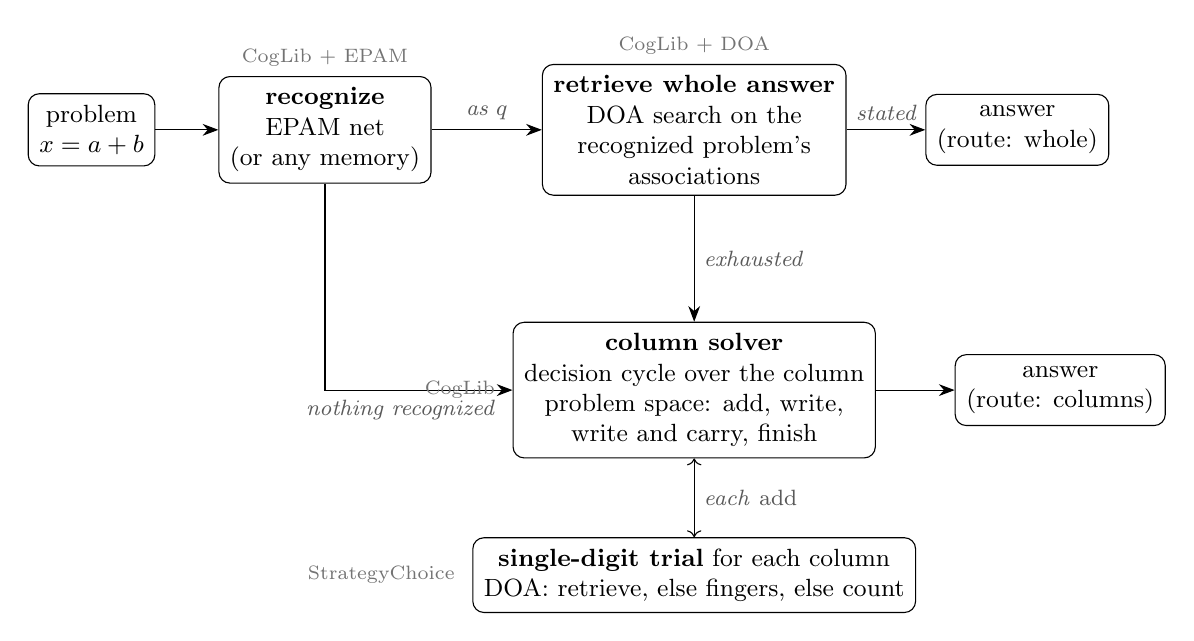
\begin{tikzpicture}[font=\small,
  box/.style={draw, rounded corners, minimum height=9mm, align=center, inner sep=4pt},
  arr/.style={-{Stealth[length=2mm]}},
  lab/.style={font=\footnotesize\itshape, text=black!65},
  src/.style={font=\scriptsize, text=black!55}]
  \node[box] (x) {problem\\$x = a+b$};
  \node[box, right=8mm of x] (rec) {\textbf{recognize}\\EPAM net\\(or any memory)};
  \node[box, right=14mm of rec] (ret) {\textbf{retrieve whole answer}\\DOA search on the\\recognized problem's\\associations};
  \node[box, right=10mm of ret] (ans) {answer\\(route: whole)};
  \node[box, below=16mm of ret] (sol) {\textbf{column solver}\\decision cycle over the column\\problem space: add, write,\\write and carry, finish};
  \node[box, right=10mm of sol] (ans2) {answer\\(route: columns)};
  \node[box, below=10mm of sol] (fact) {\textbf{single-digit trial} for each column\\DOA: retrieve, else fingers, else count};
  \draw[arr] (x) -- (rec);
  \draw[arr] (rec) -- node[lab, above] {as $q$} (ret);
  \draw[arr] (ret) -- node[lab, above] {stated} (ans);
  \draw[arr] (ret) -- node[lab, right] {exhausted} (sol);
  \draw[arr] (rec) |- node[lab, below, pos=0.7] {nothing recognized} (sol);
  \draw[arr] (sol) -- (ans2);
  \draw[arr, <->] (sol) -- node[lab, right] {each \emph{add}} (fact);
  \node[src, above=0mm of rec] {CogLib + EPAM};
  \node[src, above=0mm of ret] {CogLib + DOA};
  \node[src, left=1mm of sol] {CogLib};
  \node[src, left=1mm of fact] {StrategyChoice};
\end{tikzpicture}
\caption{One trial of the integrated model (\code{MD.Integrated.itrial}). Grey labels give the source of each mechanism. When $x$ is recognized as a familiar $q$, the whole answer is retrieved from $q$'s associations. The solver runs only when recognition fails or retrieval is exhausted, and it computes the answer from single-digit trials and a carry rule.}
\label{fig:compose}
\end{figure}

In Lean, the composition is three definitions (\code{MultiDigit/Integrated.lean}):
\begin{Verbatim}[fontsize=\small]
def solverBackup (F : Facts) (p : Problem) : Dist Nat :=
  Solver.answers F.fact Solver.full Solver.lenient p
def itrial E N str as cc n F x := trial E N str as cc n (solverBackup F) x
\end{Verbatim}
Here \code{F.fact} is the single-digit DOA trial, \code{Solver.full} the full column procedure, and \code{trial} the recognize-and-retrieve trial from \code{MultiDigit/Postulates.lean}. The integrated model introduces no new mechanism. Its only correct arithmetic knowledge is in the single-digit associations, which are peaked on each digit pair's sum, as in DOA, and in the carry rule.

\subsection{Why the integrated model is stronger evidence}

An earlier version of the example, still in the repository (\code{MultiDigit/Example.lean}), checked the general theorems with a backup that simply returned the correct sum, \code{Dist.pure p.sum}. That suffices to instantiate theorems that hold for \emph{every} backup. But it supplies the answer instead of computing it, so it is not evidence that the mechanisms compose. In the integrated model, nothing is handed the answer. The answer 250 to $150+100$ is assembled by the solver from three DOA trials and a carry rule, and it is never certain. So the composition must work at the level of mechanisms (the parts fit and run together) and at the level of theorems (the parts' results transfer to the whole).

\subsection{Composition of theorems}

Three kinds of reuse make the composition deductive rather than merely executable.

\paragraph{A bridge.} The solver on CogLib's decision cycle answers exactly as a fixed column procedure does, for every problem and every single-digit process (\lean{Solver.bridge}). Every theorem proved about the fixed procedure therefore holds for the solver. One example is that a column error is a single-digit error moved to its place (\lean{MD.column\_error\_is\_doa\_error}).

\paragraph{Associativity.} Each arrow in Figure~\ref{fig:compose} is a two-stage draw of finite distributions. CogLib proves that such draws regroup (\lean{Dist.bind\_assoc}), so a theorem about a component holds where the component sits inside the whole.

\paragraph{Well-formedness, inherited.} The general confident-errors theorem needs the backup to be a proper distribution, of total probability 1. For the integrated model this is proved, not assumed, by chaining results from three packages (\lean{mass\_solverBackup}):
\begin{itemize}
  \item DOA retrieval is proper (CogLib, \lean{mass\_search});
  \item a whole DOA trial is proper (StrategyChoice, \lean{SC.mass\_trial});
  \item the column procedure is proper when its facts are (MultiDigit, \lean{mass\_columns});
  \item the solver equals the column procedure (\lean{Solver.bridge}).
\end{itemize}
These lemmas contribute no psychology. They are what allows theorems written for an abstract backup to apply to a concrete, computing one.

\section{Derived consequences}
\label{sec:results}

We present four results, chosen because their explanatory status differs. The first is explained in detail.

\subsection{Confident errors}

In DOA alone, a problem's errors and its use of backup strategies come from the same distribution. A flat distribution of associations produces both more retrieval errors and more backup use, so errors and hesitation go together. Recognition breaks this tie. A problem confused with a familiar one is retrieved from the familiar problem's distribution: with that problem's low backup use, and with all of its answers, which are wrong for the confused problem.

The theorem, as stated for the integrated model (lightly abridged):
\begin{Verbatim}[fontsize=\small]
theorem integrated_confident_errors (E : Encoding) (N : Net) (str ...) (F : Facts)
    (hF : F.Proper) (x q : Problem) (hT : ∀ y, total as (str y) ≠ 0)
    (hq : N.select (E.code q) = some (E.code q))      -- q is recognized as itself
    (hx : N.select (E.code x) = some (E.code q))      -- x is confused with q
    (hs : Sharp str cc (E.code q) q)                  -- only q's sum clears the criterion
    (hne : x.sum ≠ q.sum) :
    prob (itrial ... q) (wholeWrong q) = 0 ∧                          -- (i)
    prob (itrial ... x) (wholeWrong x) = prob (itrial ... x) isWhole ∧  -- (ii)
    prob (itrial ... x) isColumns = prob (itrial ... q) isColumns     -- (iii)
\end{Verbatim}
In words: (i) whole-problem retrieval never errs on $q$; (ii) every whole-problem answer to $x$ is wrong; (iii) $x$ goes to the column solver exactly as often as $q$ does. The confused problem is answered wrongly with the same fluency as the familiar one.

\paragraph{What is assumed.} The postulates are the mechanisms: the net, DOA retrieval and the solver. The conditions are of three kinds.
\begin{itemize}
  \item \emph{Recognition conditions} (\code{hq}, \code{hx}): $q$ is recognized as itself and $x$ is confused with it. These are properties of a particular net. They are not arbitrary: every net EPAM learns recognizes its images as themselves (\lean{learnAll\_clean}), and the net in our setting, learned by EPAM from $100+100$ and $100+200$, is verified to confuse $150+100$ with $100+100$ (\lean{Example.net\_facts}).
  \item \emph{Sharpness} (\code{hs}): only $q$'s correct sum clears the criterion. This is an empirical premise that the library does not yet derive from learning.
  \item \emph{Well-formedness} (\code{hF}, \code{hT}): strengths have positive totals.
\end{itemize}
No hypothesis mentions confident errors, or any relation between errors and backup use.

\paragraph{What is reused.} The proof is one line. It applies \lean{MD.confident\_errors}, the theorem for an arbitrary backup, with \lean{mass\_solverBackup} for its well-formedness hypotheses. \lean{MD.confident\_errors} is in turn a relabelling of CogLib's \lean{RR.confident\_errors}, which holds for any task with problems, a familiar set and a backup. That theorem combines three earlier lemmas:
\begin{itemize}
  \item a problem recognized as a sharp $q$ gets only $q$'s answer (\lean{confusion\_gives\_neighbours\_answer});
  \item so all its whole-problem answers are wrong when the sums differ (\lean{wrong\_eq\_whole\_of\_sharp});
  \item backup use after certain recognition as $y$ is $(1-R_y)^n$, which depends only on $y$ (\lean{backup\_prob\_certain}).
\end{itemize}
The last lemma is DOA's retrieval-probability result, lifted to a recognized item.

\paragraph{Generalizing over memories.} The same pattern is proved from laws of memory instead of from a particular net (\lean{RR.confident\_errors\_of\_laws}). Any memory with three properties produces confident errors whenever a stranger can be taken for a studied item with sharp associations:
\begin{itemize}
  \item \emph{determinacy}: retrieval calls up a single item for certain;
  \item \emph{certainty}: a studied item retrieves itself;
  \item \emph{stability}: studying one item does not change another's retrieval of itself.
\end{itemize}
This is a result about a class of models, not about one model.

\subsection{Whole-problem errors do not depend on the solver}

Once $x$ is recognized as $q$, the chance of a whole-problem answer with any property is that of retrieval on $q$'s associations, whatever the backup (\lean{whole\_independent\_of\_solver}). This is a general consequence of the composition, at every setting. Its psychological content is a prediction about intervention: improving column skill, for instance by teaching carrying, cannot reduce errors that arise from mistaken recognition. Only learning that changes recognition or associations can.

\subsection{Two sources of error}

Under the same conditions as confident errors, the integrated model distinguishes two sources of error on a confused problem (\lean{errors\_two\_sources}).
\begin{itemize}
  \item \textbf{Whole-route errors} are always the confused neighbour's answer (here 200), whenever that route is taken.
  \item \textbf{Column-route errors} occur with probability equal to the chance that retrieval is exhausted times the solver's own error rate on $x$. The solver's errors are single-digit DOA errors, displaced to their column: off by $10^j\delta$ when column $j$ errs by $\delta$ (\lean{solver\_error\_is\_doa\_error}).
\end{itemize}
The two sources leave different signatures: a whole-route error is another familiar problem's sum, while a column-route error differs from the correct answer in one digit. This result is \emph{compositional}. Neither recognition nor DOA says it alone, and it would not hold with the old backup, which never erred. The model also says when the column route is exact: only when every column's single-digit trial is exact (\lean{solver\_exact\_of\_exact}). DOA sampling does not guarantee that.

\subsection{Memory substitution}

Because recognition is stated for any retriever, EPAM's net can be replaced by ACT-R's declarative memory \citep{anderson2007}, with everything else unchanged: the encoding, the associations, the criterion, the search length and the solver. CogLib implements an ACT-R-style memory with base-level activation, partial matching and a retrieval threshold, for decay 1 and temperature 1, so that probabilities stay rational (\code{CogLib/Memory/Activation.lean}).

The two memories differ in the laws just listed. Both cells are proved, for every parameter setting:
\begin{itemize}
  \item the discrimination net has determinacy, certainty and stability (\lean{Matrix.Discrimination.determinate}, \lean{.certainty}, \lean{.stability});
  \item ACT-R's memory has none of them (\lean{Matrix.Activation.never\_determinate}, \lean{never\_certainty}, \lean{never\_stability}).
\end{itemize}
So the general confident-errors theorem applies to EPAM and never to ACT-R. Its hypotheses can never be met, because nothing is retrieved for certain (\lean{Act.retrieve\_not\_certain}). Table~\ref{tab:memories} shows the consequences at one setting.

\begin{table}[t]
\centering
\small
\begin{tabularx}{\linewidth}{@{}Xcc@{}}
\toprule
& EPAM net & ACT-R memory \\
\midrule
$150+100$ retrieves $100+100$ & certainly & with probability $10/23$ \\
$150+100$ answered 200 by whole-problem retrieval & $45/46$ & $225/529 \approx .43$ \\
$150+100$ answered 300 (taken for $100+200$) & $0$ & $225/1058 \approx .21$ \\
$150+100$ reaches the column solver & $1/46$ & $383/1058 \approx .36$ \\
$150+100$ answered correctly (250), by the solver & $\approx .014$ & $\approx .238$ \\
errors on the practiced $100+100$ & $0$ & $225/782 \approx .29$ \\
the same, after also studying $100+300$ & $0$ & $3375/5842 \approx .58$ \\
\midrule
for every setting (general theorems) & confident errors; & no certain retrieval; \\
& practice never disturbed & interference possible \\
\bottomrule
\end{tabularx}
\caption{The same application with two memories. All values are exact, proved in Lean (\code{ExampleACTR.lean}, \code{Integrated.lean}), at one illustrative setting: the binary-coded encoding, both memories having studied $100+100$ and then $100+200$, the same associations, criterion $1/2$, search length 1, and the same solver. ACT-R's parameters are a mismatch penalty $\mu = 1/2$ over 24 features and a failure weight $\theta = 1/10$. The last row states what holds at every setting.}
\label{tab:memories}
\end{table}

With EPAM, the confusion is certain and confident errors dominate. With ACT-R, the confusion is graded. $150+100$ can retrieve either familiar problem, or fail. It therefore reaches the solver far more often and is answered correctly about a quarter of the time. ACT-R also predicts interference: studying $100+300$ roughly doubles the errors on the practiced $100+100$ (\lean{act\_interference}). EPAM predicts none, for every net (\lean{MD.learning\_preserves\_trial}). The difference is between kinds of memory, and the laws say which property of memory produces it.

\section{Three kinds of results}
\label{sec:kinds}

Table~\ref{tab:kinds} sorts the results of this section by what they rest on. The distinction matters for credibility. A reader should be able to tell which statements are claims about a whole class of models, which are claims given particular conditions, and which are only numbers at chosen settings.

\begin{table}[t]
\centering
\small
\begin{tabularx}{\linewidth}{@{}p{0.2\linewidth}Xp{0.27\linewidth}@{}}
\toprule
Kind & Results & What they rest on \\
\midrule
\textbf{General}: hold for every encoding, net, strength set and DOA setting & the solver equals the column procedure; whole-problem errors are independent of the solver; the column route factors as exhaustion times the solver; a solver error is a single-digit error moved to its column; the solver is a proper distribution & the mechanisms alone (plus positive strengths, for the last) \\
\addlinespace
\textbf{Conditional}: hold given stated conditions & confident errors; two sources of error; exactness of the solver only given exact facts; confident errors for any memory with three laws & recognition conditions (derivable for EPAM nets, verified for the learned net); sharp associations (an unexplained empirical premise); for the last, the laws themselves \\
\addlinespace
\textbf{At chosen settings}: exact values & $150+100$: 200 by retrieval $45/46$; solver reached $1/46$; solver correct $\approx .656$; correct overall $\approx .0143$; the ACT-R column of Table~\ref{tab:memories} & an encoding, a learned net, associations, criterion and search length chosen for illustration \\
\bottomrule
\end{tabularx}
\caption{The integrated model's results, by kind. Lean names are in Appendix~\ref{app:index}.}
\label{tab:kinds}
\end{table}

\paragraph{The illustrative setting.} The encoding codes each digit of each addend in four bits. The net is learned by EPAM from $100+100$ and $100+200$, scanning hundreds digits first, so it tests only the bit where those two problems differ. The whole-problem associations give strength $.90$ to each familiar problem's correct sum and $.01$ to other answers, with criterion $.50$ and search length 1. Every digit pair has the same single-digit associations: $4/5$ on its sum, $3/25$ on the next number in the counting sequence, and $1/100$ on each other answer from 0 to 19. The single-digit criterion is $1/10$, the search length 1, and finger elaboration, skipping and double-counting are each $1/20$.

At this setting, $150+100$ is answered 200 by whole-problem retrieval with probability $45/46$ and reaches the solver with probability $1/46$. The solver alone answers 250 with probability $\approx .656$. Its main errors are 260, 350 and 251, each $\approx .1$: a tens error, a hundreds error (the counting-sequence neighbour of $1+1$) and a units error. So $150+100$ is answered correctly with probability $\approx .0143$ (\lean{setting\_routes}, \lean{setting\_solver\_x}, \lean{setting\_overall\_x}). The familiar $100+100$ is answered correctly with probability $\approx .993$.

These numbers are exact consequences of the setting, and they show that the conditional theorems' hypotheses can be met by a learned net. They are \emph{not} fitted to children's data and are not predictions about children. Computing them required a small addition to the library. The DOA counting process, written out as a list of outcomes, lists $3^k$ of them, too many for the kernel to evaluate. A merged evaluator, proved to be the same distribution (\lean{SC.same\_trialMerged}, \lean{same\_fastBackup}), makes the computation take seconds while every value remains a probability of the model itself.

\section{The scientific status of proofs}
\label{sec:status}

\paragraph{Validity is not empirical adequacy.} A proof establishes that a conclusion follows from its premises. It does not establish that the premises are true of people. Confident errors follow from CogLean's formalization of EPAM and DOA. Whether children make them, and whether they make them for this reason, are empirical questions.

\paragraph{Validity is not explanation either.} For a theorem to be an explanation, its premises must characterize mechanisms independently, and not restate the phenomenon. An earlier version of CogLib's serial-position result illustrates the difference. Its mechanism was a schedule on which item $i$ was learned on trial twice its distance from the nearer end. Proving that this produces a bowed error curve was valid, but the bow was in the definition. The current version derives the order of learning from a rule over any set of anchors: items nearer an anchor are attended first. The same rule then has a second consequence, the isolation (von Restorff) effect, when a distinctive item serves as an anchor (\code{CogLib/Control/Serial.lean}). The result is still close to its premises. But one mechanism now answers to two phenomena, which is a real test.

The repository records an explicit audit of this kind for its headline results (\code{notes/EXPLANATORY\_AUDIT.md}). It sorts each result by how far it lies from its premises:
\begin{itemize}
  \item \emph{definitional}: a restatement of the definitions;
  \item \emph{close}: the pattern is largely in the mechanism;
  \item \emph{derived}: it follows from premises that do not mention it;
  \item \emph{compositional}: it needs two or more mechanisms working together.
\end{itemize}
Not every CogLean theorem is a psychological explanation, and we do not claim that. Some are properties of algorithms: the soundness of means-ends search, or the merge properties of semantic networks. Those are needed library facts, but they explain nothing on their own. Some are relations between laws. Some, such as confident errors, the two sources of error and solver independence, are compositional: no single mechanism contains them. Making these distinctions visible is part of the method. Lean shows every premise of every theorem; what remains is a scientific judgment, and the right place for it is written down, in the open.

\paragraph{Premises still unexplained.} The audit also lists what is assumed but not yet derived:
\begin{itemize}
  \item sharp associations, in every confident-errors result;
  \item the prior associations of the worked cases;
  \item which items serve as anchors in serial learning.
\end{itemize}
These are the library's most important targets.

\section{Checking the formalization}
\label{sec:sim}

Lean guarantees that the theorems follow from the definitions. It does not guarantee that the definitions say what the prose model says. We tested that link with an independent implementation that could not simply copy the first \citep[cf. N-version programming,][]{avizienis1985}.

\paragraph{Method.} The model was written as a prose specification, with no Lean names, theorems or predictions (\code{MultiDigit/sim/SPEC.md}). Points the prose leaves open were listed for the implementer to settle and document. Before any simulator existed, a list of checks was committed (\code{PREREG.md}). Each check named a theorem, the observable statistic, the hypothesis as read from the simulator's logs, and a tolerance: zero violations for exact relations, and frequencies within $4\sigma$ for probabilities. A check whose hypothesis never arose was to be reported as vacuous, not as passed. A fresh AI agent, given only the specification and working in an empty directory, wrote the simulator. An audit of its tool calls showed that it read only files it had written. Lean exported exact trial distributions for four instances, and a harness ran the checks on 30 random fixed instances and 20 random learning instances.

\paragraph{Agreement.} Every check whose hypothesis arose passed, with no failures. 243 outcome frequencies matched Lean's exact distributions. The predictions about routes, confident errors, carrying, column errors, zeros and thresholds, and learning (non-interference, discrimination, then column work) passed on hundreds to hundreds of thousands of tests each. The simulation predates the problem solver. Because the solver is proved equal to the column procedure the simulation implements (\lean{Solver.bridge}), its results carry over.

\paragraph{What the simulation found that the proofs did not.} Three findings remain open in the current library.
\begin{enumerate}
  \item \textbf{Unreachable hypotheses.} Five predictions (near misses within 200 or 20, round problems, and column facts) were vacuous: their hypotheses never held in any net EPAM learned. Each needs a path to test \emph{every} feature of a digit or column. EPAM grows one test per confusion, so paths are short. The theorems are true but say little about the nets the learning mechanism actually produces. Proof alone did not reveal this. Counting how often each hypothesis arose did. The distinction is between logical correctness and \emph{reachable} model states.
  \item \textbf{A gap at zero strength.} With associations of total strength 0, sampling divides by zero, and a trial has total probability 0. The theorems avoid the case by assuming positive totals. The simulator, reading the prose, treats it as exhausted retrieval, which is the natural reading.
  \item \textbf{An unstated assumption decides a predicted learning sequence.} The combined model suggests a sequence: a confident error, then, after discrimination, slow column work, then fluent correct retrieval. Whether it occurs depends on the initial associations of a newly discriminated problem, which the prose left open. With none, 40 of 48 discriminated problems followed the sequence. With only the correct answer, the column phase was skipped. With a copy of the neighbour's associations, the error was stated, strengthened and stated again: 7 of 44 problems were trapped, and 35 were still mixed at the end. The blind implementer flagged this dependence from the specification alone.
\end{enumerate}

The simulation does not prove the formalization faithful to the intended theory. It supplies independent evidence that the formal model behaves as its prose describes, and it found where the formal model says too little. Three standards are involved, and they are different: logical correctness (Lean), behavior over reachable states (simulation), and empirical adequacy (data about people), which neither addresses.

\section{Discussion}
\label{sec:discussion}

\subsection{Relation to previous formal work}

CogLean is not the first formalization or mechanical verification of a cognitive theory. Formal specification of cognitive architectures goes back at least to a specification of Soar in Z \citep{milnes1992}. It covered the architecture completely but at a low level, and it could not be executed. Cooper, Fox, Farringdon and Shallice argued that better theories would come from languages designed for specifying cognitive models, and gave one, Sceptic, an executable specification language in which they implemented several models, including Soar \citep{cooper1996}. Stewart and West rebuilt ACT-R in order to separate its core commitments from implementation detail and to explore alternative components \citep{stewart2007}. That anticipates CogLean's interest in interchangeable mechanisms, in an executable setting. Ragni and colleagues proposed a formal framework into which architectures such as ACT-R and Soar can be embedded for comparison \citep{ragni2018}.

For ACT-R in particular, Gall and Frühwirth gave an abstract operational semantics, a translation to Constraint Handling Rules proved sound and complete with respect to it, and a decidable confluence test \citep{gall2018,gall2017confluence}. Langenfeld, Westphal and Podelski translated ACT-R models to timed automata for exhaustive defect analysis \citep{langenfeld2019}, and proved their timed-automaton semantics correct at the level of architectural components \citep{langenfeld2021}. Macklem and Mili proposed specification languages and algorithms for checking cognitive models against requirements \citep{macklem2006}. In the context of the Common Model of Cognition \citep{laird2017}, Ganeriwala and colleagues have proposed enabling formal verification of cognitive models \citep{ganeriwala2025}. They have also compiled Soar models to discrete-time Markov chains for probabilistic model checking in PRISM \citep{ganeriwala2026}, which addresses stochastic behavior, as CogLean's exact distributions do. Outside architectures, verbal theories have been formalized as logic programs \citep{rohner2021} and as communicating automata \citep{finkel2025}. Fisher and colleagues derived critical tests of ACT-R from its core architectural assumptions, as theorems over a space of model classes \citep{fisher2025}, an aim close to CogLean's separation of what follows from a theory's core.

What is distinctive in CogLean, relative to this work, is a combination of emphases. Few of them are entirely new on their own:
\begin{itemize}
  \item \textbf{Theorems over classes of models}, not properties of one model's executions. Model checking establishes properties of every run of a given model. CogLean's theorems quantify over every encoding, net, strength set and backup, and, through laws, over every memory.
  \item \textbf{Phenomena and laws stated theory-neutrally}, so that rival mechanisms can be tested against the same statement.
  \item \textbf{Reusable proofs across independently developed theories.} The previous work formalizes one architecture or model at a time. CogLean's central example composes theorems proved separately for EPAM, DOA and a problem solver into results about their combination.
  \item \textbf{Behavioral predictions derived from composition}, with their premises sorted into postulates, conditions and settings.
\end{itemize}
Whether any single one of these is novel is a matter for a more complete review. The combination, in one cumulative library, is what we claim to be new.

\subsection{What the approach bought}

\paragraph{Composition as deduction.} The integrated model's predictions follow from results already proved for its parts, with a small number of new lemmas. The proofs say what each prediction rests on. For example, confident errors need the criterion and search length not to depend on the route. A failed empirical test of confident errors would therefore point at specific premises, not at the model as a whole.

\paragraph{Discovery.} Formalization and composition produced results the original authors did not state:
\begin{itemize}
  \item a dissociation between errors and backup use that neither theory produces alone;
  \item the independence of recognition errors from solver quality;
  \item a counterexample to an informal claim of the DOA chapter;
  \item hypotheses that are true but unreachable by the learning mechanism;
  \item an unstated assumption on which a predicted learning sequence depends.
\end{itemize}
The comparison of memories adds conditions under which two theories diverge, explained by laws.

\paragraph{Proof and simulation are complementary.} The slogan ``simulation explores, proof settles'' understates the relation. Simulation also checks what the proofs are \emph{about}: whether their hypotheses arise, and whether the definitions say what the prose says.

\subsection{Limitations}

\begin{itemize}
  \item The associative strengths in the worked example are chosen, not derived from experience. Siegler and Shrager's priors came from a counting process. Grounding these in learning histories is open.
  \item The strongest results depend on sharp associations and on particular recognition confusions. Confusions are derived for learned nets; sharpness is not.
  \item Single-digit DOA assumes that a representation with the right number of objects is available for elaboration and counting.
  \item Carrying is error-free in the full procedure, and columns are added independently.
  \item The framework does not establish psychological plausibility. That remains a matter of evidence and judgment.
  \item Scalability is a serious question. CogLean uses exact rational distributions over finite outcome spaces. Continuous representations, large state spaces and neural models will need different techniques, and exact evaluation already required a merged evaluator here.
  \item Three findings of the simulation remain open: unreachable hypotheses, the zero-strength gap, and the initial associations of a newly discriminated problem.
\end{itemize}

\subsection{Future work}

Natural next steps:
\begin{itemize}
  \item derive associative distributions from learning histories, so that sharpness becomes a theorem;
  \item add feedback-driven learning across whole trials, so that the predicted learning sequence can be proved;
  \item restate the vacuous predictions in terms of the features a net actually tests;
  \item generalize the retriever interface, so that more memories can be swapped in;
  \item compose theories in other domains.
\end{itemize}
The library already contains early work on the last of these: conceptual combination, semantic memory and view application, on a shared semantic-network representation.

\subsection{Conclusion}

The question was whether theories represented in a common formal library can be composed to yield meaningful consequences that would otherwise require building a new model from scratch. In one case the answer is yes. EPAM's recognition, DOA's retrieval and strategy choice, and a decision-cycle problem solver, each formalized on its own, compose into a model of three-digit addition with no answer supplied. Its predictions, confident errors, solver independence and two sources of error, are proved by reusing the components' theorems. Replacing one memory with another changes the predictions in ways that laws of memory explain. The larger ambition is a cumulative theoretical science, in which cognitive constructs and their proved properties are reused across models, tasks and research traditions, as mathematical results are reused in Mathlib. One example does not establish that. It shows that the approach can produce results of the right kind.

\paragraph{Code.} All definitions and theorems are in the CogLean repository \citep{coglean}, \url{https://github.com/jeffshrager/CogLean}. Every theorem is fully proved, with no \code{sorry}, and depends only on Lean's standard axioms.

\bibliographystyle{unsrtnat}
\bibliography{refs}

\appendix
\section{Index of results}
\label{app:index}

\begin{table}[h]
\centering
\small
\footnotesize
\begin{tabularx}{\linewidth}{@{}>{\raggedright\arraybackslash}p{0.36\linewidth}>{\raggedright\arraybackslash}X@{}}
\toprule
Claim & Lean name (file) \\
\midrule
Discrimination learning preserves prior recognition & \lean{learn\_preserves} (\code{CogLib/Process/DiscriminationLearning}) \\
A confusion agrees on every tested feature & \lean{confusion\_agrees\_on\_path} (\code{CogLib/Memory/DiscriminationNet}) \\
Learned nets recognize each image as itself & \lean{learnAll\_clean} (\code{CogLib/Process/DiscriminationLearning}) \\
DOA retrieval use, error share, backup independence & \lean{SC.retrieval\_prob}, \lean{retrieval\_error\_share}, \lean{retrieval\_independent\_of\_backup} \\
Counting errors independent of associations & \lean{SC.counting\_error\_share} \\
Peaking can raise overt strategy use & \lean{SC.peaking\_can\_raise\_overt\_use} \\
Confident errors, any task & \lean{RR.confident\_errors} (\code{CogLib/Process/RecognizeRetrieve}) \\
Confident errors from laws of memory & \lean{RR.confident\_errors\_of\_laws} \\
Solver equals the column procedure & \lean{Solver.bridge} (\code{MultiDigit/Solver}) \\
A column error is a DOA error in place & \lean{MD.column\_error\_is\_doa\_error} (\code{MultiDigit/Columns}) \\
Integrated: solver is the column backup; proper & \lean{solverBackup\_eq\_columns}, \lean{mass\_solverBackup} (\code{MultiDigit/Integrated}) \\
Integrated: whole-problem errors independent of solver & \lean{whole\_independent\_of\_solver} \\
Integrated: column route factored & \lean{columnsSuch\_prob} \\
Integrated: confident errors; two sources & \lean{integrated\_confident\_errors}, \lean{errors\_two\_sources} \\
Integrated: solver error is a DOA error; exact only given exact facts & \lean{solver\_error\_is\_doa\_error}, \lean{solver\_exact\_of\_exact} \\
Integrated: values at the setting (EPAM; ACT-R) & \lean{setting\_routes}, \lean{setting\_solver\_x}, \lean{setting\_overall\_x}, \lean{setting\_overall\_q1}; \lean{setting\_actr\_x} \\
ACT-R: graded confusion; interference & \lean{act\_values}, \lean{act\_interference} (\code{MultiDigit/ExampleACTR}) \\
EPAM: practice never disturbed & \lean{MD.learning\_preserves\_trial} \\
Memory laws: EPAM has, ACT-R never has & \lean{Matrix.Discrimination.*}, \lean{Matrix.Activation.never\_*} (\code{CogMatrix}) \\
Merged evaluation is the same distribution & \lean{SC.same\_trialMerged}, \lean{same\_fastBackup} \\
\bottomrule
\end{tabularx}
\end{table}

\end{document}
